\documentclass[12pt,letterpaper]{article}

% Essential packages
\usepackage[utf8]{inputenc}
\usepackage[margin=1in]{geometry}
\usepackage{graphicx}
\usepackage[x11names,table]{xcolor}
\usepackage{setspace}
\usepackage{float}
\usepackage{caption}
\usepackage{authblk}
\usepackage[backend=biber,style=numeric]{biblatex}
\usepackage{doi}
\usepackage{url}

% Minimal code chunk support
\usepackage{fancyvrb}
\usepackage{framed}
\definecolor{shadecolor}{rgb}{.97, .97, .97}
\newenvironment{Shaded}{\begin{snugshade}}{\end{snugshade}}
\newenvironment{Highlighting}{}{}

% Bibliography settings
\addbibresource{references.bib}

% Document settings
\doublespacing
\setlength{\parindent}{0.5in}

% Title formatting - ASM style
\renewcommand{\Affilfont}{\normalfont\normalsize}
\renewcommand{\Authfont}{\normalfont\normalsize}

% Section numbering
\renewcommand{\thesection}{\arabic{section}.0}
\renewcommand{\thesubsection}{\arabic{section}.\arabic{subsection}}

% Headers
\usepackage{fancyhdr}
\pagestyle{fancy}
\fancyhf{}
\renewcommand{\headrulewidth}{0pt}
\fancyhead[R]{\thepage}

% Lists
\providecommand{\tightlist}{%
  \setlength{\itemsep}{0pt}\setlength{\parskip}{0pt}}

% Hyperlinks (last)
\usepackage{hyperref}
\hypersetup{
    colorlinks=true,
    linkcolor=black,
    filecolor=black,
    urlcolor=black,
    citecolor=black
}

\begin{document}

% Title
\title{Group Task 3: Hurricane Risk Assessment for Gulf of Mexico
Cities}

% Hardcoded authors section - ASM style
\author{Yves-Langston Mays}\affil{Department of Natural Sciences \& Mathematics, University of Houston Main Campus, Houston, USA\\\texttt{ymmays@cougarnet.uh.edu}}
\author{Uyen Vi Phan}\affil{Department of Natural Sciences \& Mathematics, University of Houston Main Campus, Houston, USA\\\texttt{uphan2@uh.edu}}
\author{Ny Dang}\affil{Department of Natural Sciences \& Mathematics, University of Houston Main Campus, Houston, USA\\\texttt{tndang8@cougarnet.uh.edu}}

\date{\today}
\maketitle

% Abstract
\begin{abstract}
Task 3 centers on hurricane risk for 25 cities in the Gulf of Mexico,
using data from the Atlantic hurricane database (HURDAT2) from 1851 to
2023, provided by the National Hurricane Center. To analyze and assess
this risk, we will perform 3 analyses in R to assess the hurricane risk
on the Gulf of Mexico. First, we visualize and note our findings on the
storm tracks over the last 25 years (1999-2024), focusing on storm
paths, intensity, and duration at each location. Spatial correlation
analysis will be used to explore the relationship between hurricane
occurrences and contributing environmental factors, while Non-Parametric
Density Estimation will estimate location-specific risk based on
historical hurricane trajectories. These analyses collectively aim to
identify the cities at highest risk of hurricane impact and gauge
potential severity.
\end{abstract}

% Table of Contents
\tableofcontents
\newpage

\section{1.0 Introduction}\label{introduction}

One of the most common natural disaster plaguing the Gulf of Mexico are
Hurricanes. Just this year (2024) there has been 9 hurricanes in the
Atlantic Ocean including Beryl, Helen and Milton. These storms can have
lasting impacts to people's lives, the environment, infrastructure and
to the economy. Since 1980, hurricane damage has costed over \$1.3
trillion in damages with an average of \$22.8 billion dollars per event
and 6,890 deaths {[}1{]}. Learning to predict where, when, and the
intensity of hurricanes can not only save us billions of dollars but
thousands of lives as well. This is especially important for cities that
are at high risk such as cities like New Orleans that exists at
extremely low elevations.

This task aims to use historical data on hurricanes to predict future
hurricane activity and highlight cities that are at most risk. The
historical hurricane data from the National Hurricane Center's HURDAT2
database, contains hurricane data in the Atlantic from 1851 to 2023.
HURDAT2 records the six-hourly information on the location, maximum
winds, central pressure, and (beginning in 2004) size of all known
tropical cyclones and subtropical cyclones{[}2{]}. Along with a list of
25 cities and their locations in the Gulf of Mexico, 3 analyses will be
performed oh HURDAT2 to analyze and predict the storm tracks in the Gulf
of Mexico.

The last 25 (1999-2024) years worth of storm tracks will be first
visualized and analyzed on the over the Gulf of Mexico to identify
common patterns and trends of the storm tracks. The visualization and
the manual analysis provides a good general overview of how these storms
move, where they are the most intense, and what places receive the most
storms.

The second analysis examines how certain factors like sea surface
temperatures and El Nino/La Nina patterns affect hurricane activity.
Spatial correlation analysis between these factors and hurricane
activity will be used to achieve this. The correlation analysis will
show how certain weather phenomena can affect hurricane activity to
better predict hurricane activity.

The last analysis uses non-parametric density estimation to assess the
hurricane risk based on past trajectories and severity. This can provide
insight on where hurricanes are more likely to appear and what routes
they take. It can assess what regions will receive the most intense
storms. Paired with the spatial correlation analysis, the information
provided from the non-parametric density estimation can highlight what
cities are most at risk in the Gulf of Mexico.

These 3 analyses can provide valuable insight to the behavior and
activity of future hurricanes. Knowing the behavior and patterns of the
hurricanes, knowing what cities and regions are at the most risk from
hurricane activity and how different factors play a role in hurricane
activity can help people better prepare for hurricanes and minimize the
losses caused by these storms. Meteorologists can use these predictions
to better inform people about the route, severity of storms and what to
expect as it passes. Governments can use this information to predict
what cities will require the most aid. Insurance companies can use this
data to decide what services are best suited to a specific location.

This task aims to use historical data on hurricanes to predict future
hurricane activity and highlight cities that are at most risk. The
historical hurricane data from the National Hurricane Center's HURDAT2
database, contains hurricane data in the Atlantic from 1851 to 2023.
HURDAT2 records the six-hourly information on the location, maximum
winds, central pressure, and (beginning in 2004) size of all known
tropical cyclones and subtropical cyclones {[}2{]}. Along with a list of
25 cities and their locations in the Gulf of Mexico, 3 analyses will be
performed oh HURDAT2 to analyze and predict the storm tracks in the Gulf
of Mexico.

The last 25 (1999-2024) years worth of storm tracks will be first
visualized and analyzed on the over the Gulf of Mexico to identify
common patterns and trends of the storm tracks. The visualization and
the manual analysis provides a good general overview of how these storms
move, where they are the most intense, and what places receive the most
storms.

The second analysis examines how certain factors like sea surface
temperatures and El Nino/La Nina patterns affect hurricane activity.
Spatial correlation analysis between these factors and hurricane
activity will be used to achieve this. The correlation analysis will
show how certain weather phenomena can affect hurricane activity to
better predict hurricane activity.

The last analysis uses non-parametric density estimation to assess the
hurricane risk based on past trajectories and severity. This can provide
insight on where hurricanes are more likely to appear and what routes
they take. It can assess what regions will receive the most intense
storms. Paired with the spatial correlation analysis, the information
provided from the non-parametric density estimation can highlight what
cities are most at risk in the Gulf of Mexico.

These 3 analyses can provide valuable insight to the behavior and
activity of future hurricanes. Knowing the behavior and patterns of the
hurricanes, knowing what cities and regions are at the most risk from
hurricane activity and how different factors play a role in hurricane
activity can help people better prepare for hurricanes and minimize the
losses caused by these storms. Meteorologists can use these predictions
to better inform people about the route, severity of storms and what to
expect as it passes. Governments can use this information to predict
what cities will require the most aid. Insurance companies can use this
data to decide what services are best suited to a specific location

\section{2.0 Background}\label{background}

Background stuff here

\section{3.0 Methodology}\label{methodology}

\subsection{3.1 Data Collection and
Preparation}\label{data-collection-and-preparation}

\subsection{3.2 Geographic Data Setup}\label{geographic-data-setup}

\begin{verbatim}
Study Area Boundaries:
\end{verbatim}

\begin{verbatim}
Latitude: 16.5 to 31.7 °N
\end{verbatim}

\begin{verbatim}
Longitude: -98.9 to -76.4 °W
\end{verbatim}

\begin{verbatim}

Total storm observations: 13669
\end{verbatim}

\begin{verbatim}

Unique storms: 961
\end{verbatim}

\begin{verbatim}

Date range: 18510625 to 20230830
\end{verbatim}

\subsection{3.3 Visualization}\label{visualization}

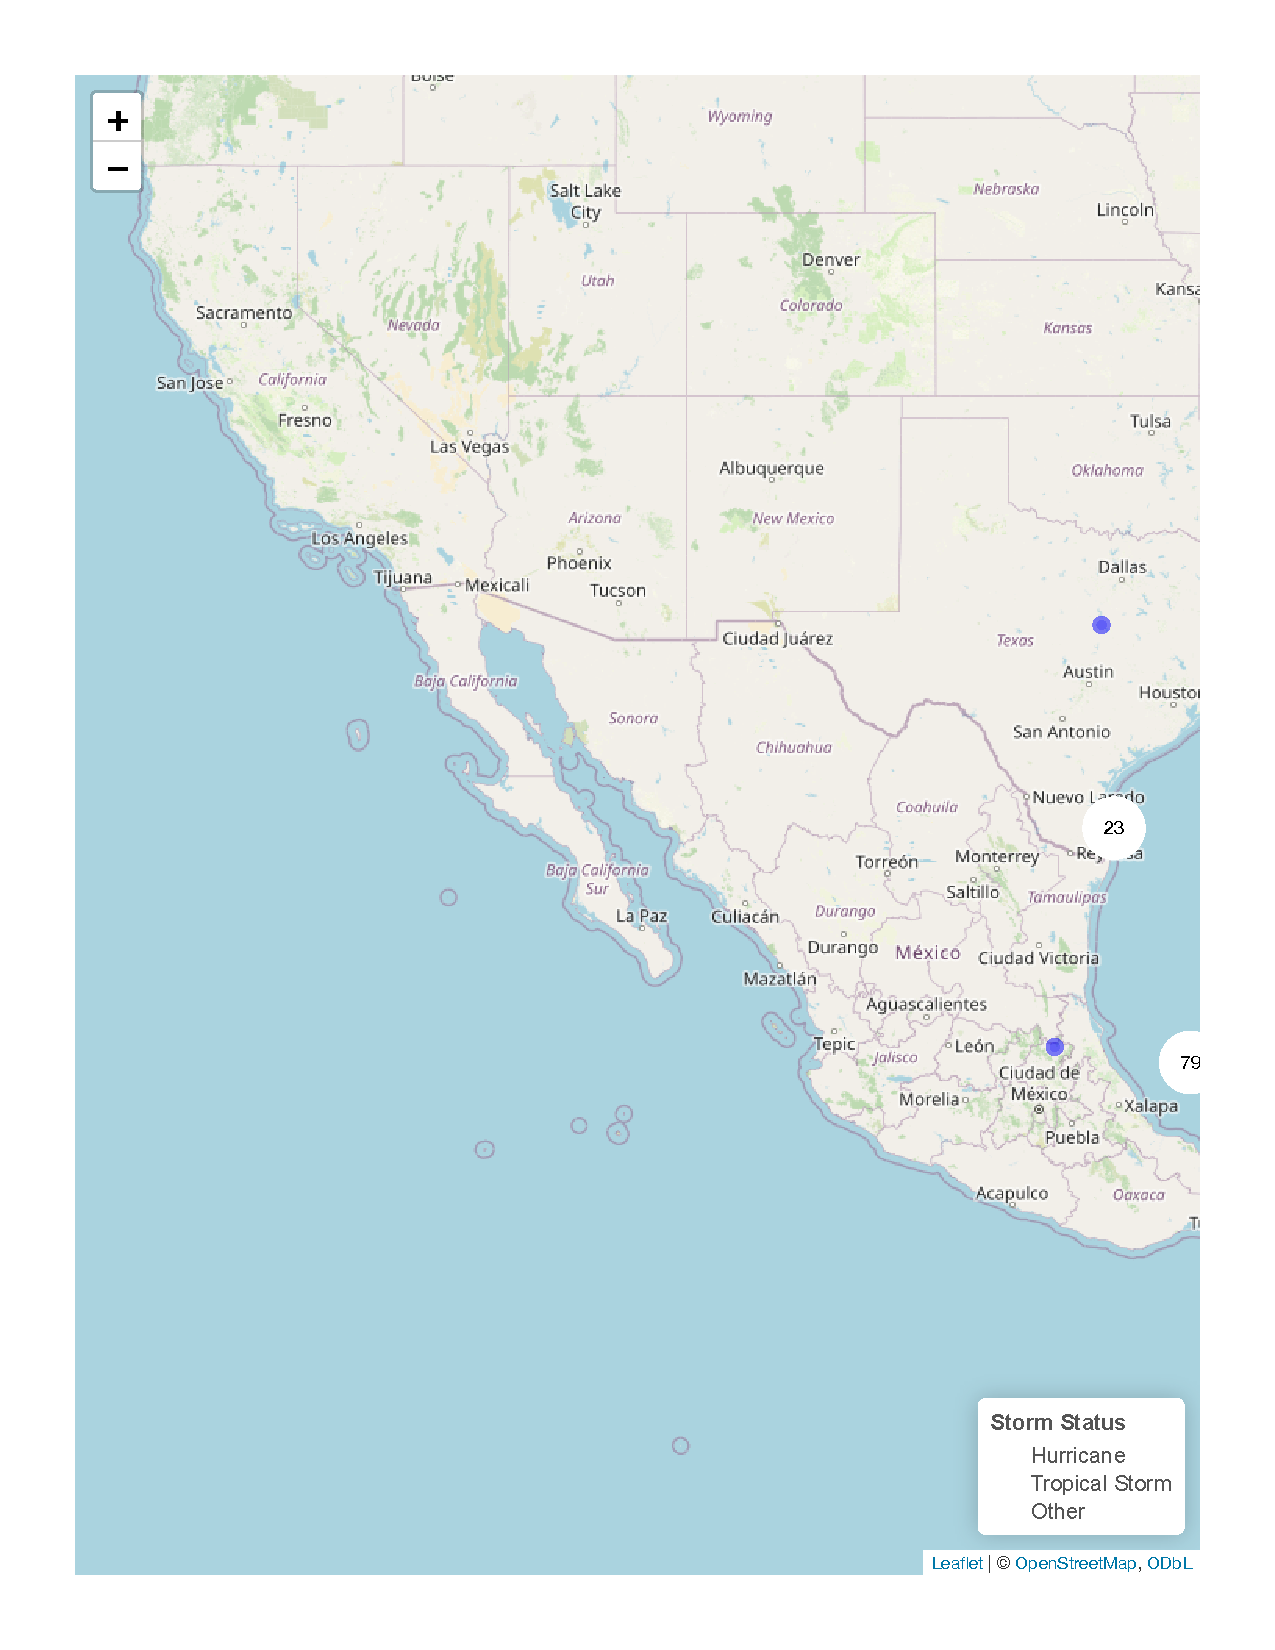
\includegraphics{GroupTask3_files/figure-pdf/LeafletMap-1.pdf}

\subsection{3.4 Statistical Analysis}\label{statistical-analysis}

\begin{verbatim}
ggplot(yearly_storms, aes(x = YEAR, y = storm_count)) +
  geom_line(color = "blue") +
  geom_point() +
  labs(title = "year storm count from 99-23",
       x = "Year",
       y = "# of Storms")
\end{verbatim}

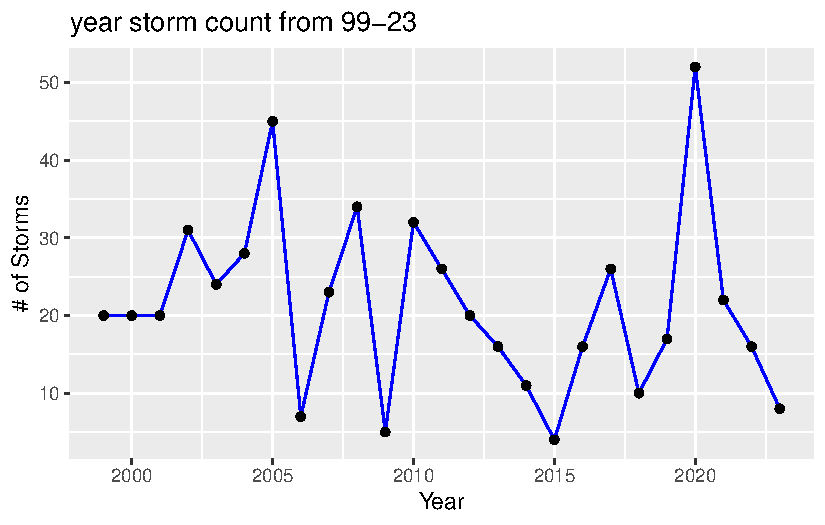
\includegraphics{GroupTask3_files/figure-pdf/Plots-1.pdf}

\begin{verbatim}
ggplot(monthly_storms, aes(x = MONTH, y = storm_count)) +
  geom_col(fill = "steelblue") +
  labs(title = "monthly storm freq",
       x = "Month",
       y = "# of Storms") +
  scale_x_continuous(breaks = 1:12,
                     labels = c("Jan", "Feb", "Mar", "Apr", "May", "Jun", 
                                "Jul", "Aug", "Sep", "Oct", "Nov", "Dec"))
\end{verbatim}

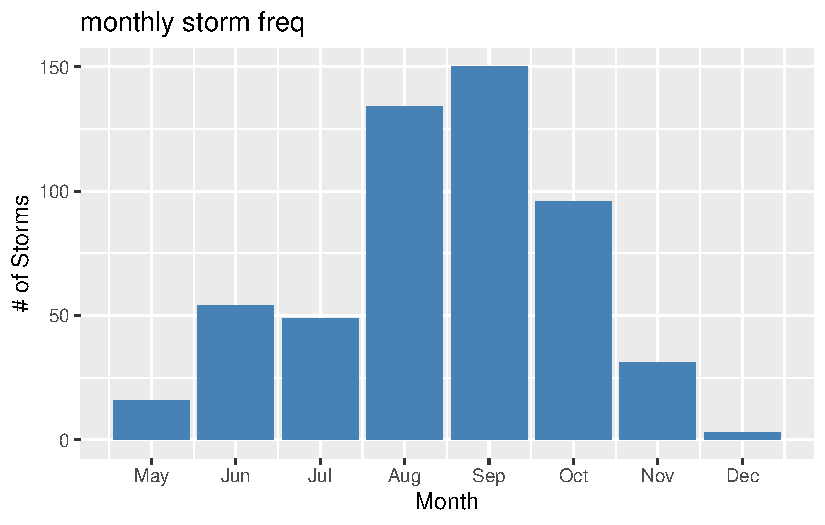
\includegraphics{GroupTask3_files/figure-pdf/Plots-2.pdf}

\begin{verbatim}
ggplot(status_count, aes(x = STATUS, y = count, fill = STATUS)) +
  geom_bar(stat = "identity") +
  labs(title = "strm count by status",
       x = "Status",
       y = "# of Storms") +
  scale_fill_manual(values = c("HU" = "red", "TS" = "orange", "TD" = "blue"))
\end{verbatim}

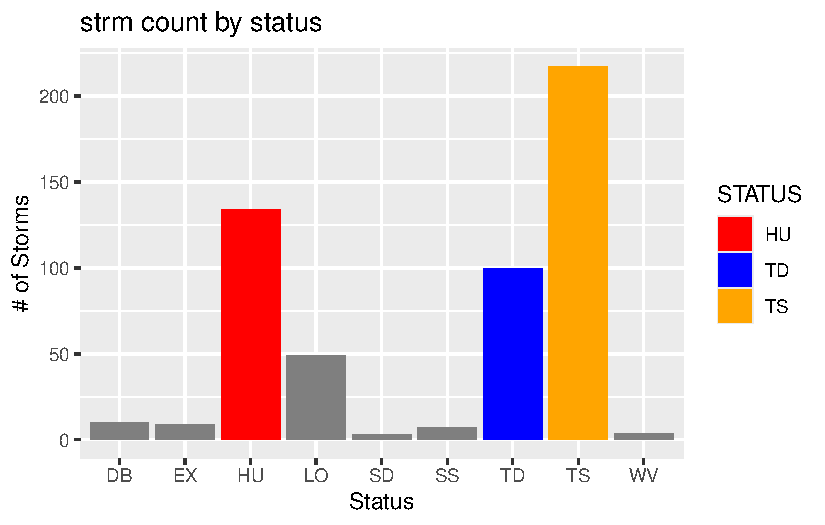
\includegraphics{GroupTask3_files/figure-pdf/Plots-3.pdf}

\begin{verbatim}
intensity_trend <- recent_gulf_storms %>%
  group_by(YEAR) %>%
  summarize(avg_windspeed = mean(WINDSPEED_KT, na.rm = TRUE))

ggplot(intensity_trend, aes(x = YEAR, y = avg_windspeed)) +
  geom_line(color = "darkred") +
  geom_point() +
  labs(title = "Avg Storm Intensity Over Time 99-23",
       x = "Year",
       y = "Avg Wind Speed (kt)")
\end{verbatim}

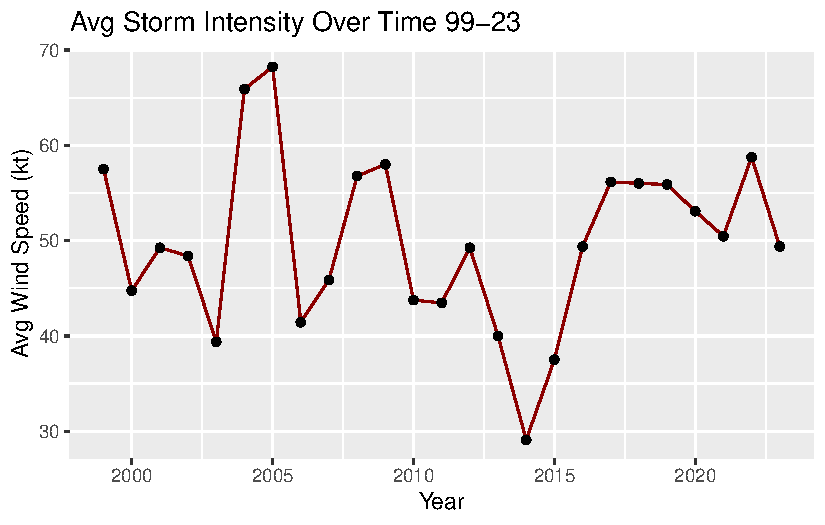
\includegraphics{GroupTask3_files/figure-pdf/Plots-4.pdf}

\newpage

\section{4.0 Results}\label{results}

Discuss results of analysis

\newpage

\section{5.0 Discussion}\label{discussion}

Discuss the implications and significance here

\newpage

\section{6.0 Conclusion}\label{conclusion}

Conclusion Here

\section*{References}\label{references}
\addcontentsline{toc}{section}{References}

\printbibliography[heading=none]

\end{document}
